%!TEX root = main.tex
\chapter{État de l'art}
\chaptertable

%\section{La visualisation et manipulation 3D collaborative sur web}

\section{Modélisation 3D collaborative sur le web}

\subsection{Collaboration et concurrence en 3D}
\label{sec:concurrence}
Dans un contexte collaboratif, on considère qu'il n'est pas possible pour une 
personne seule de réaliser la tâche proposée complètement. 
La modélisation 3D collaborative permet à différents concepteurs de travailler 
ensemble sur une même tâche de manière efficace (en terme de coûts temporel et 
financier) et avec un support visuel manipulable, éditable et flexible (proposant 
différentes possibilités de visualisation). 
En se complétant, leur travail peut aussi entrer en conflit, se compenser, 
s'annuler\ldots
Mettre en place une situation de travail collaboratif demande en plus de prendre en compte de nombreux facteurs 
comme le type de collaboration (synchrone, asynchrone) et de cohérence souhaités 
(forte, éventuelle) par exemple.

Mettre en place une situation de travail collaboratif demande en plus de prendre en compte, les différentes solutions pour la conception collaborative peuvent être divisées en 
trois types: 
\begin{enumerate*}[label=(\roman*)]
	\item les mécanismes de type autoritaire (requérant des autorisations) ;
	\item les opérations de transformation ;
	\item et les autres solutions synchrones et asynchrones.
\end{enumerate*}
Selon leur comportement face à l'apparition d'un conflit, ces types de 
collaboration sont classifiés comme pessimistes ou optimistes (Tableau 
\ref{table:collprobs}). Les solutions de type autoritaire (\og \textit{authoritative}\fg{}) 
sont comptées parmi les solutions pessimistes car elles préviennent toute 
occurrence de conflit, tandis que les solutions des deux autres types,
transformées opérationnelles -- \gls{OT} -- et autres (synchrones ou asynchrones), 
sont dites optimistes car permissives face à l'apparition de conflits. 
Dans ce dernier cas, les conflits détectés peuvent, selon les stratégies, amener à 
une résolution automatique ou manuelle.

\begin{table}
	\centering
	\noindent
	\caption{Solutions conventionnelles pour les problèmes collaboratifs 
	\cite{Yu2016}.}
	
	\small
	\label{table:collprobs}
	\begin{tabular}{ m{0.20\textwidth}  m{0.35\textwidth} m{0.35\textwidth}}\hline
		\textbf{Type}& \textbf{Mécanismes de Collaboration} & \textbf{Problème 
		résolu}    \\ \hline
		\multirow{4}{*}{Autoritaire}                     & Verrou                        & 
		\multirow{4}{*}{Évitement des conflits}                                          \\
		& Feux de circulation  
		&                                                                                  \\
		& Droits d'accès               
		&                                                                                  \\
		& Permission temporaire        
		&                                                                                  \\ \hline
		\multirow{2}{0.2\textwidth}{Transformées opérationnelles}                     & 
		Séquence de transformation                     & Résolution de conflit temps réel 
		pour les documents textuels                     \\ \cline{2-3} 
		& Transformées opérationnelles 3D                 & Résolution de conflit pour  des modèles 3D                              \\ \hline
		\multirow{3}{0.2\textwidth}{Autre (synchrone ou asynchrone)} & 
		Semi-synchrone                               & \multirow{3}{0.3\textwidth}{Détection 
		de conflit ou résolution avec interaction utilisateur} \\
		& Signalisation des conflits %(conflict awareness) 
		&                                                                                  \\
		& Résolution de conflit créative                 &                      \\ 
		\bottomrule                                                           
	\end{tabular}
\end{table}


La plupart du temps, ce sont des mécanismes autoritaires comme le mécanisme 
de verrouillage (\textit{lock mechanism}), des feux de circulation (\textit{traffic 
light mecanism}) requérant des droits ou des permissions temporaires, qui sont 
proposés dans les solutions collaboratives traditionnelles. Les utilisateurs doivent 
souscrire aux permissions du système avant de pouvoir effectuer leurs 
modifications. Ces mécanismes permettent de s'assurer que les opérations sont 
effectuées de manière séquentielle, ce qui assure la cohérence des données à 
travers le système. Plus simples à mettre en place, ces mécanismes sont aussi plus 
restrictifs vis-à-vis de la liberté de création des utilisateurs du système. Par 
exemple, Lets3D \cite{Ha2015} est un éditeur collaboratif 3D sur le web dont la 
gestion de la concurrence repose sur la demande de permission par objet 
sélectionné (ce qui verrouille l'objet pour les autres utilisateurs lorsqu'elle est 
accordée).

 Avec ceux d'Ellis et Gibbs, les travaux de Greenberg et Marwood sont parmi les 
premiers à s'intéresser aux problèmes liés à la gestion de la concurrence dans 
un système distribué au sein d'un collecticiel \cite{Ellis1989,Greenberg1994}. 
L'\gls{EVC3D} Duplex \cite{Pacull1994}, présenté au même 
moment, s'intéresse plus spécifiquement aux problématiques de 
passage à l'échelle en essayant de réduire la taille du contexte partagé pour 
limiter les problèmes liés à la concurrence. 
Les approches pour défaire / refaire (\textit{undo/redo}) des manipulations dans 
les éditeurs collaboratifs distribués sont nombreuses. Les travaux les plus 
aboutis s'intéressant à la cohérence dans un environnement distribué collaboratif concernent les documents 
textuels \cite{Prakash1994,Ressel1996,Sun2002}. 
Les algorithmes souvent utilisés dans ce cadre sont les algorithmes 
de  transformées opérationnelles -- \gls{OT} -- \cite{Ellis1989} ou les algorithmes 
de réplication de  données commutatives -- \glspl{CRDT} -- \cite{Shapiro2007} 
s'orientant de plus en plus vers des solutions décentralisées pour un usage à 
grande échelle \cite{Weiss2009a}. 

L'existence de protocoles agnostiques\footnote{Indépendant des 
protocoles de communication, le protocole dit \og agnostique\fg{} négocie le 
protocole avec son pair et commence la communication. Cette démarche 
apporte plus de flexibilité et d'interopérabilité au système.} comme Dat 
\cite{Ogden2017} permet également une synchronisation fiable pour des 
contenus dynamiques. Dat est un protocole de synchronisation de jeu de données 
qui n'assume pas que le jeu de données soit statique ou que le jeu de données 
soit entièrement téléchargé. C'est un protocole agnostique dont la conception 
repose sur la garantie de trois principes. D'une part, l'intégrité du contenu est garanti grâce à l'utilisation de valeurs de hachage (\textit{hash}) signées. Elles sont mises à jour régulièrement de manière décentralisée (\textit{decentralized mirroring}). Cela permet de découvrir automatiquement les pairs et effectuer l'échange de données en essaim. D'autre part, le protocole impose également un chiffrement des données de bout en bout. Enfin, il propose un versionnage incrémental pour la 
synchronisation des données. Ce protocole est, par exemple, utilisé par 
hashbase.io, un service qui se propose d'être un pair toujours présent pour 
l'hébergement de sites web en \gls{P2P}, promettant ainsi une disponibilité 
pérenne du contenu. 


\subsection{... sur le web : HTML5 et au-delà}
%TODO designing in context
%\cite{Dobos2015}

L'arrivée du web a bouleversé les usages liés à la collaboration sur des objets 3D. 
Les principes, les technologies, l'omniprésence du web en ont fait une plateforme 
de prédilection pour la visualisation et la manipulation d'objet 3D de haut niveau.   
Pour les projets d'\gls{AIC} ou de \gls{BIM}, la demande de traitement et la fidélité 
ont tendance à être plus élevés, particulièrement pour la représentation de dessins 
d'ingénierie ou de modèles d'architecture 3D. 
Les objets simples (primitives) ou les maillages optimisés pour le rendu temps réel 
ne sont ni suffisants ni assez génériques pour être supportés par tous les 
processus liés à l'élaboration d'un produit. 
Plus les projets sont gros, plus ils dépendent d'une multitude de logiciels 3D --  
dont l'interopérabilité n'est pas garantie -- pourvoyant chacun aux besoins d'une 
tâche spécifique. 
Chaque tâche (ex: modélisation \gls{CAO}, \textit{stress testing}\ldots) possède sa 
propre représentation des données qui peut varier selon les niveaux de 
sémantique attachés à la géométrie. 
Pour garder une trace de ces données et mettre en commun les données 
générées autour d'un produit, l'utilisation d'un \gls{PDM}/\gls{PLM} est 
souvent requise. Certains outils de création d'objets 3D (par exemple 
Autodesk Revit) autorisent -- mais pas systématiquement -- la synchronisation de fichier via leur dépôt à distance. 
En cela, une plateforme web pour un \gls{PDM}/\gls{PLM} a 
l'avantage d'être distribuée pour être accessible depuis un navigateur web ; avec 
un système d'édition hors-ligne, le téléversement peut s'avérer long et fastidieux.
De plus, les logiciels spécialisés pour la modélisation 3D, contrairement aux jeux 
multijoueurs, sont traditionnellement dédiés à un utilisateur unique sans 
représentation visuelle des autres opérateurs dans le même espace 3D. 
Ici encore, les principes d'accessibilité du web facilitent la création d'un espace 
virtuel 3D collaboratif pour la visualisation, la manipulation et l'échange de
données partagées. 


La collaboration en temps-réel est de plus en plus présente sur le web pour 
différents types de documents, notamment 3D.
La revue sur la visualisation distribuée, effectuée par Grimstead et al. en 2005 
\cite{Grimstead2005}, indiquait que la plupart des systèmes sont conçus pour 
moins de cent 
utilisateurs simultanés et reposent sur un ou plusieurs serveurs pour supporter ces 
utilisateurs. 
Ils expliquent ce schéma par la volonté du fournisseur de service d'assurer une 
qualité de service et la sécurité du système. 

Les systèmes de \gls{RV} collaboratifs font exception à ce schéma où l'utilisation 
des réseaux \gls{P2P} est plus répandue pour supporter parfois plus d'un millier 
d'utilisateurs simultanés. 
Dans chacun des cas, chaque système a besoin d'un client adapté pour opérer de 
manière isolée, sans inter-opérer avec les autre systèmes. 
C'est dans ce contexte qu'en 2011, Mouton et al. \cite{Mouton2011} présentent 
une analyse approfondie de l'état de l'art des environnements collaboratifs 3D, ciblant 
principalement la visualisation collaborative. 
Ils montrent l'apparition de la tendance à déporter les environnements collaboratifs 
sur le web, grâce à l'évolution d'XMLHttpRequest en client-serveur et l'apparition 
du standard HTML5 comprenant un support avancé de l'audio et de la vidéo, ainsi 
que plusieurs \gls{API} de stockage côté client (LocalStorage, IndexedDB). 

De plus, les applications web revêtent plusieurs avantages par rapport aux applications 
natives sur mobiles ou aux logiciels autonomes. 
Cela repose principalement sur le fait que les navigateurs sont présents partout 
dans nos vies en 2017, incluant les téléphones intelligents et les 
tablettes qui les rendent indépendants des plateformes utilisées. 
Le déploiement sur le web ne requiert pas d'installation ou de mises à jour autres 
que celles du navigateur -- en ne considérant que les applications sans greffon (\textit{plugin less}). 
La modification de l'application est gérée de manière centralisée par les serveurs 
qui distribuent l'application. 
Les éditeurs peuvent diffuser leur application à l'échelle mondiale instantanément  
et la mettre à disposition des utilisateurs sans dépendre d'un réseau de distribution 
autre qu'internet.

%Computer-Aided Engineering (CAE) Collaborative /

Parmi les solutions sans greffon dédiée à de la modélisation 3D, de nombreuses utilisent l'architecture client-serveur et le 
protocole \gls{WebSocket} pour effectuer la synchronisation entre les différents 
clients collaborateurs. Quelques raisons peuvent expliquer cette situation. 
Historiquement, les développeurs sont plus familiers avec les architectures 
client-serveur et le standard \gls{WebSocket}. Techniquement, la gestion de 
données (la synchronisation et la gestion de la concurrence) est facilitée 
dans un \gls{EVC} avec une architecture centralisée. 
Commercialement, le suivi des données de l'utilisateur est plus simple avec un 
serveur central qui garantit un engagement de l'utilisateur vis-à-vis du service 
(voire une dépendance).


%
Le choix de plateformes web dans l'infonuagique (\og cloud\fg{}) pour la 
modélisation \gls{CAO} est prépondérant pour les solutions commerciales comme 
OnShape, Clara.io et TinkerCAD. Les fonctionnalités minimum de ces plateformes 
consistent en la mise en place d'un environnement 3D pour visualiser un objet 3D accompagnées d'un système défaire / refaire et d'une plateforme de 
diffusion des créations.
OnShape est un service de modélisation 3D très riche dont l'objectif est de 
proposer une qualité équivalente des fonctionnalités de modeleurs autonomes 
(\textit{standalone}) professionnels, le tout de manière collaborative. Leur approche 
de la gestion de version développe le concept de micro version \cite{Baran2015}. 
Cette approche est employée dans les travaux de Lu et al. \cite{Lu2016} pour 
gérer l'évolution de productions participatives liées à des tâches de modélisation 
3D en usant de la créativité, de l'intelligence et du savoir-faire 
d'un grand nombre de personnes en sous-traitance (\textit{crowdsourcing}). 
Le modeleur 3D Clara.io \cite{Houston2013} est plus généraliste. Il s'oriente 
davantage vers des fonctionnalités avancées de rendu 3D sur le \textit{cloud} en 
utilisant du lancer de rayons. 
Les fonctionnalités d'historisation et de collaboration proposées 
dans Clara.io restent très basiques (seulement annuler~/~refaire). TinkerCAD 
est aussi une plateforme de publication d'objets 3D pour faciliter l'accès à la 
conception d'objets 3D. 
TinkerCAD est une application destinée au grand 
public pour la conception et l'impression 3D. De ce fait, les fonctionnalités sont 
limitées à cause du domaine (l'impression 3D) et de la cible (le grand public). La gestion 
de version est donc plus légère, similaire à celle proposée par Clara.io. 
OpenJSCAD, Verold Studio, Vectary sont d'autres 
exemples de modeleurs 3D moins connus, avec des fonctionnalités proches de 
TinkerCAD.
%Un peu à part, GrabCAD est une plateforme web plus orientée sur la gestion de 
%données 3D \gls{CAO} (\gls{PLM}), qui possède un système de gestion de 
%version 
%performant et un système d'annotation et de visualisation collaboratives.
Pour réduire l'empreinte mémoire des messages transmis lors de la collaboration 
sur le web, certains systèmes d'édition collaborative de contenu 3D utilisent une 
modélisation par surfaces implicites (BlobTree) \cite{Grasberger2013}. 
Les objets sont alors manipulés comme des géométries de construction de 
solides avec les opérations booléennes associées. Le tableau \ref{table:encoding} 
résume les différents types 
d'encodages associés aux types de modélisation~3D. 

\begin{table}[h]
	\centering
	\caption{Encodage des données transmises}
	\label{table:encoding}
	\begin{tabular}{@{}lcc@{}}\hline
		\textbf{Référence}& \textbf{Modélisation 3D}   & 
		\begin{tabular}[c]{@{}l@{}}\textbf{Encodage des}\\ 
			\textbf{modifications}\end{tabular} \\ \midrule
		\cite{Grasberger2013}        &      Blob (CSG)    & Fonction implicite        \\
		Clara.io \cite{Houston2013}               & Polygonale       &  Commande 
		interface     \\
		\cite{Mouton2014}                  & Polygonale       & Fonction paramétrique     \\
		OnShape \cite{Baran2015} &    Paramétrique      &     Microversion    \\
		cSculpt \cite{Calabrese2016} &      Polygonale    &    Fréquence spatiale  \\ 
		\bottomrule
	\end{tabular}
\end{table}
%\improve{tableau comparatif gestion historique ou versionning}
%\improve{tableau comparatif de GrabCAD, OnShape, clara.io}
%\begin{table}[]
%	\centering
%	\caption{Comparaison de fonctionnalités entres modeleurs 3D basés web}
%	\label{my-label}
%	\begin{tabular}{@{}cccc@{}}
%		&  Client serveur & P2P &  Collaboratif\\ \midrule
%		Claro.io        & c        & g       & o       \\
%		GrabCAD                  & c        & g       & o       \\
%		OnShape &          &         &         \\
%		&          &         &         \\ \bottomrule
%	\end{tabular}
%\end{table}
\subsection{Web 3D : deux approches}
La plateforme web possède certains avantages par rapport à des clients lourds. 
En effet, l'essor de l'infonuagique a permis le développement de 
meilleures infrastructures de services. Ces dernières ont rendu faisable, en termes de ressources, mais également en termes de 
technologies la création de 
plateformes collaboratives sur le web pour faire de la conception 3D.

Il existe deux types d'approches pour créer du contenu web 2D ou 
3D : l'approche déclarative et l'approche impérative. La Figure \ref{fig:impdec} 
montre le pendant 3D pour chaque approche 2D. En 2D, les spécifications 
déclaratives (\gls{SVG}) et impératives (canvas) sont issues du dernier standard HTML (HTML5), alors qu'en 3D, les spécifications sont encore en évolution. 

\begin{figure}[hbt]
	\centering
	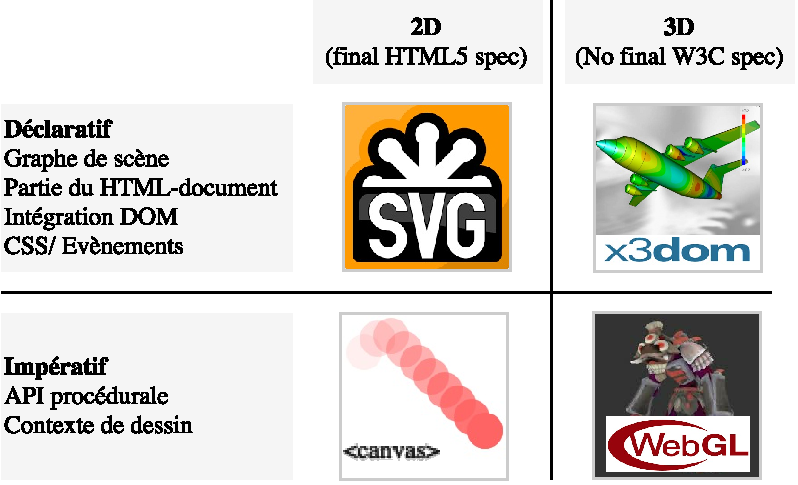
\includegraphics[width=0.8\columnwidth]{impdec}
	\caption{Déclaratif vs Impératif en 2D et en 3D sur le web}
	\label{fig:impdec}
\end{figure}

L'approche déclarative (Dec3D) s'intègre au \gls{DOM} et se 
focalise sur l'utilisation de technologies du web existantes comme CSS3, 
HTML5 et l'Ajax. 
X3D est ainsi un format de fichier respectant le standard ISO \cite{X3D2011} permettant de 
représenter des scènes 3D interactives en XML et rétro-compatible avec VRML97. Il 
se différencie des formats de fichiers comme Collada en intégrant le comportement de 
la scène durant l'exécution en plus de la description du contenu 3D. Les deux 
bibliothèques les plus notables dérivées de ce standard sont X3DOM 
\cite{Behr2010} et XML3D \cite{Sons2010} : toutes les deux sont capables de 
supporter les récentes avancées de WebGL pour afficher une scène décrite dans 
le \gls{DOM} à l'intérieur d'un \textit{canvas} HTML5. 
X3DOM essaye de respecter le standard X3D et ses concepts pour que le format s'intègre au \gls{DOM}. De plus, X3DOM intègre le support 
d'éléments \gls{HTML}, les événements \gls{DOM} et de profils \acrshort{CSS} en 
supplément \cite{Sutter2015}. 
En comparaison avec X3DOM, XML3D a développé une extension à \gls{HTML}5 
pour décrire une scène 3D. 
L'utilisation d'un langage déclaratif comme X3D s'adapte bien à des contextes où le XML est très présent (exemple : \gls{SIG}) : le contenu 3D peut être directement transformé (ex. XSLT) d'une 
représentation à une autre (tout comme le X3D peut être rendu dans un navigateur 
en utilisant X3DOM). 

L'approche déclarative est utilisée dans de nombreux travaux de visualisation 
scientifique 3D distribuée \cite{Jung2012}, par exemple, pour des données spatiales 
\cite{Stein2014} ou du rendu volumique \cite{Becher2012}. 
En manipulant directement les objets 3D à partir des éléments \gls{DOM}, grâce à 
sa structure bien connue, il est alors plus simple, lors de la collaboration, d'utiliser 
ces éléments \cite{Gadea2016} ou les événements du \gls{DOM} \cite{Lowet2009} 
comme protocole de synchronisation de scènes. 
L'ajout de nombreux \textit{listeners} sur un document peut affecter les 
performances de parcours de l'arbre du \gls{DOM} notamment si une scène est
très peuplée.
%declarative XML- based languages such as X3D are suited well for SOAs in that 
%3D content, such as CAD/ CAM data or a given WCS response in a GIS 
%application, can be directly transformed, e.g. via an XSLT or similar transform, 
%from one representa- tion to another (such as an X3D world that can be rendered 
%in 
%real-time in the web browser using the X3DOM frame- work).

%TODO BIM CAD PLM 
%TODO Building Information Modeling: The Web3D Application for AEC 
%\cite{Campbell2007}
%TODO WEB3D, COLLABORATIVE DESIGN AND PLM Enrico Vezzetti (1), 
%Maria Grazia Violante (2)
%\info{webrtc collaborative visual analysis \cite{Li2015} }
%\info{webrtc medical \cite{Andrikos2015}}
%\info{webrtc x3dom \cite{Stein2014} \cite{Andrioti2015} }
%\info{webrtc webgl \cite{Desprat2015} \cite{Desprat2016} SAGE2 
%\cite{Marrinan2008} }

\begin{figure}[hbt]
	\centering
	\includegraphics[width=0.9\columnwidth]{webglstats.eps}
	\caption{Support de WebGL 1 (2014-2017) et WebGL 2 
		(2016-2017)}
	\label{fig:webglstats}
\end{figure}

Concernant l'approche impérative, la spécification WebGL 1.0 \cite{Khronos2011} 
proposée par le groupe Khronos permet aux navigateurs d'effectuer un rendu 3D 
grâce à une \gls{API} JavaScript adaptée de l'\gls{API} d'OpenGL~ES~2.0 
\cite{Khronos2007} en utilisant l'élément \textit{canvas} d'\gls{HTML}5. Cette 
spécification est supportée par la plupart des navigateurs traditionnels (Chrome 
depuis v49, Firefox depuis v52, Safari depuis v9.1, IE 11\footnote{Le contexte 
	WebGL est accessible depuis <<~\texttt{experimental-webgl}~>> au lieu de 
	<<~\texttt{webgl}~>>.\label{fn:webglcontext}}, Edge 14\textsuperscript{ 
	\ref{fn:webglcontext}} et Opera depuis v41) ainsi que les navigateurs mobiles 
	(iOS 
Safari depuis v9.3, Android Browser depuis v53 et Chrome for Android depuis v53) 
à l'exception d'Opera Mini\footnote{Données issues de 
	\url{http://caniuse.com/\#search=webgl}, consulté le 26/11/2016.}. La 
	spécification 
WebGL 2.0 \cite{Khronos2016} basée sur OpenGL~ES~3.0 \cite{Khronos2008}, 
déjà publiée en tant que brouillon, est en phase 
expérimentale\footnote{\url{http://caniuse.com/\#feat=webgl2} consulté le 
	26/11/2016}.\improve{add some example of coviz web} La Figure 
\ref{fig:webglstats} montre l'évolution du support de WebGL~1 et WebGL~2 durant 
ces dernières années sur les différentes plateformes possédant un navigateur 
web\footnote{Images capturées sur \url{https://webglstats.com/}. Les statistiques 
	sont collectées à partir de sites partenaires de \url{webglstats.com}. Ces sites 
	ciblent des néophytes de WebGL possédant  en général le matériel 
	dédié à la 3D. Consulté le 04/07/2017.}.

\section{Communication en temps-réel}
L'expression temps-réel est largement utilisée par des applications requérant une 
forme de temps de réponse rapide et réactif pour que l'utilisateur ait une bonne 
expérience. La communication dans un \gls{EVC} est primordiale pour échanger entre les collaborateurs. Elle doit respecter l'intention des utilisateurs pour leur permettre de s'immerger dans la collaboration et faire confiance à l'application (exactitude des modifications).

L'exigence vis-à-vis des temps de réponse est  
grande et ce pour deux raisons principales : les limitations humaines (mémoire et 
attention limitées 
à court terme) et les aspirations de l'être humain (besoin d'être en contrôle sur les 
machines). S'accroissant au gré de la technologie et des attentes des 
utilisateurs (rétro-compatibilité, temps de 
chargement), cette exigence varie selon le domaine : elle est prépondérante sur le 
web en général. 
Par exemple, dans un domaine connexe comme le e-commerce, une étude réalisée 
en 2009 explique qu’une grande partie des internautes abandonneraient leurs achats 
en ligne si les pages mettaient 2 secondes ou plus à charger\footnote{\url{https://www.akamai.com/us/en/about/news/press/2009-press/akamai-reveals-2-seconds-as-the-new-threshold-of-acceptability-for-ecommerce-web-page-response-times.jsp}}. De nos jours, ce 
délai a été réduit au quart de seconde pour les grandes entreprises du web. Jakob 
Nielsen \cite{Nielsen1993a} indique quatre valeurs limites concernant les 
temps de réponses :
\begin{itemize}
	\item \textit{0,1 seconde} donne une sensation de réponse instantanée, comme 
	si le 
	résultat avait été produit par l'utilisateur et non l'ordinateur. Ce niveau de temps 
	de réponse soutient la sensation de manipulation directe.\footnote{En IHM, la 
		manipulation directe correspond à un mode d'interaction au cours duquel les 
		utilisateurs font des actions sur les objets d'intérêt affichés dans l'interface 
		utilisateur en utilisant des actions physiques, incrémentales et réversibles 
		dont 
		les effets sont immédiatement visibles sur l'écran.} 
	\item \textit{1 seconde} garde le flux de pensées de l'utilisateur sans 
	interruption. 
	L'utilisateur peut ressentir un délai et par conséquent savoir que c'est la 
	machine qui génère le résultat ; il a quand même une impression de 
	contrôle sur l'expérience générale et peut se déplacer librement dans l'interface 
	sans attendre la machine. Ce degré de réactivité est impératif pour une bonne 
	navigation.
	\item \textit{10 secondes} conserve l'attention de l'utilisateur. Entre 1 et 10 
	secondes, l'utilisateur se sent dépendant de la machine, mais peut faire avec. 
	\item \textit{Au delà} de 10 secondes, l'utilisateur va commencer à penser à autre chose, rendant difficile 
	le retour à la tâche une fois que la machine répond.
\end{itemize} 
Dans le domaine de l'édition et la manipulation collaborative 
d'objets 3D, les contraintes abordées se situent à divers degrés : au chargement 
et lors des mises à jour. Le chargement concerne la phase de téléchargement des ressources (page web, modèles 3D), parfois lourdes. Cette phase peut tolérer des délais relativement longs (1-10s) compte tenu du fait que l'utilisateur 
connaît en partie les contraintes liées à la taille des objets 3D. 
Concernant les mises à jour, l'édition 
collaborative requiert un temps de réponse raisonnablement court qui est contraint par 
l'exactitude des calculs et le temps dans lequel le résultat est produit. Pour les 
mises à jour internes -- produites par l'utilisateur, actions sur l'interface -- on 
s'accordera dans cette thèse sur un délai inférieur à 0,1 seconde. 
Pour les mises à jour externes -- produites par les collaborateurs -- les latences 
réseaux rentrent en compte (serveur, pairs\ldots), et on s'accordera sur un délai 
entre 1 et 10 secondes selon les degrés d'asynchronicité possibles. 





La communication et la transmission des données lors de la collaboration comptent parmi les piliers d'un \gls{EVC3D}. Que ce soit dans dans un 
\gls{EV}, un jeu multijoueur ou un jeu sérieux (\textit{serious game}), les 
participants interagissent en (quasi) temps réel, alors qu'ils sont situés à 
différents endroits géographiques. 
Le développement d'un \gls{EVC3D} nécessite donc des connaissances issues de 
plusieurs domaines comme la conception et l'implémentation de protocoles 
réseaux et de réseaux distribués.

Un protocole de communication en temps-réel existe, il s'appelle \gls{RTP} et a 
été développé dans le but de faciliter la communication en temps-réel sur un 
réseau. Coexistant avec \gls{RTP}, le protocole \gls{RTCP} est utilisé pour 
transmettre des informations de contrôle à propos des données en temps-réel. 
\gls{RTCP} transporte des données contenant des informations de contrôle et des 
informations statistiques concernant les flux de données et les connexions des 
destinataires qui permettent à l'expéditeur d'ajuster le flux en conséquence. Les 
protocoles \gls{RTP} et \gls{RTCP} sont principalement conçus pour la 
transmission de flux audio et vidéo, moins pour des données arbitraires comme 
des données 3D. Pour cette raison, leur utilisation est limitée dans le cadre des 
\gls{EVC} pour la modélisation 3D. 

La variété des domaines et applications auxquels s'adressent les 
\glspl{EVC3D} actuels fait qu'il n'existe pas de protocole de 
communication parfait, adapté à tous les types d'environnements. 
Les besoins en communication, qui se formulent souvent en termes de 
fiabilité de la livraison des messages et de l'ordonnancement des messages, sont 
les variables d'ajustement en fonction des contraintes qu'imposent les limites de 
temps de réponse et de bande passante.

\subsection{Fiable versus Non Fiable}
\label{sec:fiabilite}
La fiabilité d'un protocole de communication définit comment le protocole fait face 
à la perte ou au retard de données. Un protocole dit \og fiable\fg{} (\textit{reliable}) 
fait en sorte de rendre sûr le fait que le destinataire recevra éventuellement les 
données envoyées par l'expéditeur. Lors de la perte d'un paquet, ou lorsqu'il est 
retenu quelque part dans le réseau, le protocole est au courant et essaye de 
renvoyer les données concernées. Un protocole dit \og non fiable\fg{}, ne fournit 
pas ce genre de garantie et n'essaiera pas de transmettre à nouveau les données.

Bien que la fiabilité dans une communication soit une propriété habituellement 
recherchée, elle implique également que le canal doive connaître l'état des données 
qui transitent. Dans le cas où l'expéditeur numérote les paquets en séquence, seul le destinataire a la connaissance des paquets manquants (et à 
renvoyer). Pour indiquer les paquets manquants à l'expéditeur, le destinataire peut 
envoyer des acquittements (ACKs) pour confirmer leur réception. Ces ACKs 
peuvent être joints aux messages ou envoyés séparément. En plus des données 
additionnelles envoyées, un protocole fiable peut aussi générer des latences 
sévères (dans l'attente d'un paquet perdu ou avec beaucoup de retard). Cela peut 
impliquer que les \og nouvelles\fg{} données peuvent arriver et être déjà 
périmées.

Pour certaines applications qui ne peuvent pas faire face à ces délais potentiels 
ou ne peuvent pas se permettre l'utilisation de données additionnelles, les protocoles non fiables 
sont utilisés. 
L'expéditeur se repose alors sur le réseau pour délivrer les paquets 
correctement, mais il n'y a aucune garantie. Les protocoles non fiables ne 
nécessitent pas de données additionnelles (séquence de nombre ou ACKs). 
L'expéditeur n'est cependant jamais sûr que le destinataire a reçu toutes les 
données envoyées. Lorsque le destinataire a une connaissance du type de trafic qu'il reçoit, 
il peut fournir un retour à l'expéditeur pour qu'il ajuste le flux de paquets. Ce 
principe est appliqué par le protocole \gls{RTCP}, conjointement avec \gls{RTP}, 
pour fournir les données statistiques liés à la  connexion à l'expéditeur.

L'utilisation d'un protocole de communication fiable ou non fiable dépend du 
type d'application et du type de l'environnement réseau dans lequel il est conçu 
pour opérer. Si une application dite temps-réel est conçue pour fonctionner en réseau 
local -- \gls{LAN} -- l'utilisation d'un protocole fiable est une option recommandée. 
Les câbles utilisés dans ce contexte sont souvent rapides et stables ; un paquet 
perdu ou corrompu peut rapidement être détecté et retransmis. Dans des 
environnements réseaux moins prévisibles comme les \gls{MAN} ou 
\gls{WAN}, la nature de l'application a une influence importante sur le type de 
protocole à utiliser. Selon si la pertinence des données est de courte durée, ou si 
la perte de données n'est pas aussi importante que le fait de la retarder, alors un 
protocole non fiable peut être employé.


\subsection{Ordonné versus Désordonné}
\label{sec:ordre}
Les paquets envoyés par l'expéditeur ne prennent pas forcément tous le même 
chemin vers l'expéditeur. La réaction des réseaux face à la congestion consiste à 
modifier les tables de routage afin que les paquets évitent le n\oe ud congestionné. 
Cela peut altérer l'ordre des paquets à la réception. Le choix du protocole a 
également une influence sur la gestion de l'ordre d'arrivée des paquets.

Les protocoles dits \og ordonnés\fg{} garantissent que l'ordre dans lequel les 
paquets sont envoyés est préservé dans l'application, lors de la réception de ces 
données par le destinataire. Même si les paquets arrivent dans le désordre, le 
protocole peut imposer l'ordonnancement des données à l'aide d'une mémoire 
tampon en attendant les données précédentes. Cela impose que le protocole 
(comme pour un protocole fiable) numérote les paquets ou utilise un estampillage 
pour connaître l'ordre. Cependant, la fiabilité n'est pas nécessaire pour la livraison 
dans l'ordre. Par exemple, dans une conversation vidéo, si une image met trop de 
temps à arriver, elle sera mise en tampon, puis omise au-delà d'une limite (taille 
tampon ou temps).

Forcer à la fois la fiabilité et l'ordonnancement peut causer des latences du côté 
du destinataire, même lorsqu'une grande partie des données est déjà reçu. Quand 
un des premiers paquets est perdu ou en retard mais que d'autres données ont 
déjà été reçues, ces données doivent attendre avant d'être livrées, tant que le 
paquet n'est pas arrivé. Les communications non ordonnées sont plus simples à 
gérer car les données sont délivrées dès qu'elles arrivent. Cela signifie également 
que la numérotation des paquets n'est pas requise (paquets plus légers). 
L'application est alors en charge de gérer le fait que les paquets arrivent dans le 
désordre. La livraison de paquets ordonnés est souvent une fonctionnalité 
appréciée dans le 
cadre des \gls{SEC}. C'est particulièrement le cas en 3D afin de respecter l'intention de l'utilisateur, car l'ordre des actions en détermine le résultat. Par 
exemple, le calcul deux rotations consécutives se traduit par la multiplication deux matrices 3D qui n'est pas commutatif.

\subsection{Les principaux protocoles de transport}
Les principes de fiabilité et d'ordonnancement décrits plus haut sont souvent 
utilisés pour discriminer les différents protocoles de communication. En ce qui concerne les 
applications en temps-réel, ces principes sont considérés comme les aspects les plus 
importants à considérer pour le choix d'un protocole de communication. La 
présentation succincte des protocoles ci-dessous indique leur propriété de 
fiabilité et d'ordonnancement.
\subsubsection{TCP}
Le \gls{TCP} est probablement le protocole le plus utilisé sur internet pour 
transporter des données : navigation web, chat, transfert de fichiers\dots 
\gls{TCP} est un protocole dit \og orienté connexion\fg{}, ce qui implique que les 
deux terminaux sur le réseau s'informent et s'accordent chacun sur ce qu'ils 
veulent envoyer / recevoir de la part de l'autre. 
Quand cet accord est établi, la connexion \gls{TCP} est ouverte et le flux peut 
transiter par la connexion. 
\gls{TCP} envoie des données sous forme de flux continu d'octets qui arrivent de 
manière fiable et ordonnée. 
L'application peut lire les données à partir de ce flux.

\gls{TCP} a également un champ de somme de contrôle (\textit{checksum}) afin 
de vérifier les données dans les cas d'erreurs (mauvais signal, routeur 
défectueux). 
Si la somme est incorrecte, la données est écartée et considérée comme perdue. 
Une nouvelle copie de la donnée est alors attendue à la réception lorsque 
l'expéditeur détecte qu'il n'a pas reçu le ACK concernant la donnée erronée.

\subsubsection{UDP}
Le \gls{UDP} est considéré comme l'opposé de \gls{TCP} concernant plusieurs 
aspects. Premièrement, \gls{UDP} ne nécessite pas, pour établir la connexion, d'étape 
de configuration et d'accord comme \gls{TCP}. Les deux terminaux doivent 
configurer un \textit{socket} \gls{UDP} et écouter ce \textit{socket} pour récupérer 
les données entrantes. 
Du fait qu'aucun accord n'est établit par les deux terminaux, chacun 
peut envoyer ou recevoir des données de n'importe quel \textit{socket} proprement 
configuré.
Deuxièmement, \gls{UDP} est un protocole dit \og orienté message\fg{}. Par 
rapport à \gls{TCP} où il n'y a pas de distinction claire entre les messages du fait 
de sa nature (flux continu), \gls{UDP} fait une distinction claire entre chaque 
message (un message envoyé donne un message reçu, sauf si perte du 
message). Les messages qui transitent en \gls{UDP} sont envoyés de manière 
non fiable et désordonnée. L'en-tête \gls{UDP} n'a pas de notion de numérotation, il 
est plus léger que \gls{TCP} à cet égard.

\gls{UDP} n'a pas de champ pour faire une somme de contrôle pour détecter les 
potentielles erreurs dans un paquet. Cependant, cette fonctionnalité est optionnelle 
dans IPv4 qui rapport une somme de contrôle remplie de zéros en cas d'erreur. En 
IPv6, la somme de contrôle est obligatoire ; donc même si \gls{UDP} est non fiable, 
il doit fournir les moyens de vérifier les paquets pour la fiabilité de 
la transmission.

Même si \gls{UDP} n'est ni fiable et ni ordonné, il est souvent utilisé comme 
protocole de base sur lequel d'autres protocoles viennent se greffer car il reste très 
léger. Ces autres protocoles peuvent s'assurer de l'ordonnancement et / ou de la 
fiabilité à leur manière (re-ordonnancement, retransmission\dots). 

\subsubsection{SCTP}
Le \gls{SCTP} est le plus jeune des trois protocoles présentés. Ce protocole 
emprunte des fonctionnalités à \gls{TCP} mais utilise une approche orientée 
message comme \gls{UDP}. Comme \gls{TCP}, la connexion doit être négociée 
entre les deux terminaux. \gls{SCTP} discute également le nombre de flux utilisés 
: il autorise le multiplexage de plusieurs flux de données dans une seule 
connexion \gls{SCTP}. En comparaison, \gls{TCP} sépare chaque flux dans une 
connexion différente : le support de plusieurs flux est géré à plus haut niveau.

\gls{SCTP} a été conçu comme un protocole fiable avec une option pour envoyer 
les messages de manière ordonnée ou non ordonnée. L'ordonnancement choisi est 
signifié par un \textit{bit-flag} dans l'en-tête associée au message. Une extension 
du protocole permet de configurer la fiabilité d'un message expédié. La fiabilité 
partielle peut être établie en fonction de différents paramètres (temps d'attente ou 
nombre de tentatives 
avant retransmission). Cependant, seul l'expéditeur est au courant du niveau de 
fiabilité des données. Lorsque le destinataire remarque des données manquantes, 
il envoie à l'expéditeur des acquittements sélectifs (SACKs). Un SACKs contient 
les séquences de messages reçus et manquants et c'est à l'expéditeur de vérifier 
la configuration de la fiabilité des messages. Pour les messages marqués non 
fiables, l'expéditeur génère un nouveau paquet pour notifier le destinataire qu'il 
peut les \og oublier\fg{} et avancer sa séquence de nombre à la valeur données 
dans le nouveau paquet. 

Le champ de vérification de somme dans l'entête \gls{SCTP} est deux fois plus 
grand que pour \gls{UDP} ou \gls{TCP} : 32 bits. Cela est dû au support des 
fonctionnalités comme le multiplexage qui introduit de nombreuses sous entêtes 
par exemple.

L'adoption de ce protocole est ralentie par le fait que l'implantation de \gls{SCTP} 
n'est pas supportée par tous les systèmes d'exploitation notamment 
Windows \cite{Hogg}. 

\begin{table}[h]
	\caption{Aperçu des procotoles de transport}
	\noindent\small
	\begin{tabular}{cccc}
		& \textbf{Fiabilité} & \textbf{Ordonnancement} & \textbf{Error-free} \\ 
		\hline 
		\textbf{TCP} & Oui & Oui & Oui \\ 
		\hline 
		\textbf{UDP} & Non / À plus ht niveau & Non / À plus 
		ht 
		niveau & Opt. 
		(IPv4) / 
		Oui (IPv6) \\ 
		\hline 
		\textbf{SCTP} & Configurable & Configurable &  Oui \\ 
		\hline
	\end{tabular} 
\end{table}

\subsection{Web et P2P : WebRTC}
\label{sec:webrtc}
Le développement de la communication en \gls{P2P} sur le web a 
débuté en 2011 avec les premiers brouillons du standard \gls{WebRTC} proposé 
par le \gls{W3C} et l'\gls{IETF}\textsuperscript{\textregistered}. 
\gls{WebRTC} est une technologie qui fournit aux navigateurs web la possibilité de 
communiquer en temps-réel (\textit{Real-Time Communications}) via une collection 
de standards, protocoles et \glspl{API} JavaScript (Figure \ref{fig:protocolstack}). 
L'un des atouts de cette technologie est de permettre de façon simple et 
sans module d'extension la capture d'un flux audio et / ou vidéo (ex : 
applications de VoIP), ainsi que l'échange de données arbitraires entre 
navigateurs sans nécessiter d'intermédiaires (ex : partage de fichier en 
P2P).


Techniquement, \gls{WebRTC} supporte un canal temps-réel 
bidirectionnel pour l'échange de données. Contrairement à 
\gls{WebSocket}, qui est basé sur \gls{TCP}, \gls{WebRTC} se base sur 
\acrshort{UDP} en intégrant une pile de plusieurs protocoles (Figure 
\ref{fig:protocolstack}) qui lui offre des fonctionnalités similaires (fiabilité, 
ordonnancement, sécurité). 


Plusieurs projets impliquant les protocoles proposés par \gls{WebRTC} 
se sont intéressés à l'\gls{API} \textit{MediaStream} (flux continus audio 
et vidéo) mais très peu utilisent la partie dédiée au transfert de données 
\textit{DataChannel}. 
Selon le site officiel de WebRTC\footnote{\url{https://webrtc.org}}, plus d'un milliard 
d'utilisateurs ont utilisé la technologie \textit{open source} WebRTC. Ericsonn Labs 
a été parmi les premiers à implémenter une application WebRTC en 2011. 
La jeunesse du protocole (2011) fait que peu de travaux académiques 
l'utilisent pour créer des \gls{EVC3D} \cite{Desprat2015a,Steiakaki2016} et 
optimiser le partage de modèles 3D \cite{Koskela2014}. 
Côté commercial, un grand nombre d'applications et de services 
basés sur ce protocole ont fait leur apparition (par ordre d'importance) : 
des systèmes d'échanges audio / vidéo (VoIP)\footnote{WebRTCWorld en 
	liste un peu plus de 140 
	\url{http://www.webrtcworld.com/webrtc-list.aspx}. Consulté le 
	07/07/2017.}, des systèmes de partage de fichiers\footnote{WebTorrent 
	\url{https://github.com/feross/webtorrent}. Consulté le 04/09/2017.} et 
autres applications (capture d'écran, réalité augmentée, jeux)
\footnote{Curation de ressources et modules WebRTC 
	recensant plus de 100 projets 
	\url{https://github.com/openrtc-io/awesome-webrtc}. Consulté le 
	07/07/2017.}. WebRTC se retrouve également dans le domaine de l'optimisation 
	de l'utilisation des ressources pour la création de \glspl{CDN} 
	\cite{Zhang2013b}, de grilles de calcul comme dans
	browserCloud.js \cite{Dias2015a} ou pour faire des analyses visuelles 
	collaboratives dans un environnement hétérogène \cite{Li2015}.


L'utilisation et la gestion de réseaux \gls{P2P} sont des changements de paradigme 
qui peuvent représenter une 
barrière d'entrée auprès des développeurs web, habitués aux architectures 
client-serveur. 
Cependant, l'implantation de WebRTC, très semblable à WebSocket, rend la 
technologie facilement abordable dans un premier temps. L'attrait pour les 
propriétés du \gls{P2P} (distribution, résilience) est une motivation 
supplémentaire, en plus des implications sociales que cette architecture (partage, 
coopération, coût) dressent en faveur de l'intégration de WebRTC dans les 
applications web.

Les machines clientes et les terminaux d'extrémité (\textit{end systems}) 
sont considérés comme \og les ressources\fg{} dans un réseau 
\gls{P2P}. 
En principe, ces ressources sont difficilement administrables à l'échelle 
dans un réseau non structuré ; la qualité de service peut en pâtir car la 
synchronisation est plus complexe. C'est également problématique pour simuler 
ces environnements car il n'existe pas de solution pérenne pour tester WebRTC à 
l'échelle ; chaque service doit créer son propre système de test. 
Dans un contexte industriel, il est peu probable d'être confronté à une architecture 
\gls{P2P} totalement décentralisée (sans serveur). Une solution centralisée permet 
d'utiliser la partie serveur pour télécharger l'application cliente qui contient la 
couche intergicielle \gls{P2P}. 
Les serveurs sont aussi présents pour fournir à l'utilisateur différents services (ex: 
base de données, service de signalisation). 

\begin{figure}[ht]
	\centering
	\includegraphics[width=0.8\columnwidth]{protocol_stack2.eps}
	\caption{Pile des protocoles IP: TCP vs UDP}
	\label{fig:protocolstack}
\end{figure}
\paragraph{Échange de données via RTCDataChannel}
L'\gls{API} RTCDataChannel ou Data\-Channel, issue de  WebRTC, 
permet l'échange \gls{P2P} de données arbitraires avec peu de latence et 
un bon débit sur la base des sessions RTCPeerConnection.
DataChannel utilise de multiples canaux simultanés avec une gestion de 
priorité. L'\gls{API} est aussi capable de gérer la fiabilité de la livraison des 
paquets et sécurise nativement les données avec le protocole 
\gls{DTLS}. 
Le contrôle de la congestion des flux et l'ordonnancement éventuel est 
effectué par les protocoles \gls{SCTP} et \gls{RRTCC}. 

%TODO
%\cite{Eskola}\cite{Singh2013b}

Depuis 2011, les contributeurs du standard WebRTC font beaucoup 
d'efforts pour élargir et maintenir la compatibilité et interopérabilité entre les navigateurs.
%TODO \info{parler de edge}\improve{dans CE sens}\info{parler de 
%ORTC}. 
Cependant, certains navigateurs (comme Chrome) imposent une limite de taille 
pour l'envoi de messages contenant de la donnée brute, ce qui contrevient au 
principe énoncé par le standard.
%Enfin, la sécurité des 
%communications est encore vulnérable malgré le chiffrement des données 
%par défaut (\gls{DTLS}).

\subsubsection{Mécanisme de signalisation et problématiques réseaux}
Le mécanisme de signalisation (\textit{signaling mecanism} en anglais) 
permet de coordonner et d'envoyer des messages de contrôle durant une 
session. Le mécanisme de signalisation est utilisé pour échanger trois 
types d'information : 
\begin{itemize}
	\item des messages de contrôle sur la session pour ouvrir ou fermer un 
	lien de communication et rapporter les erreurs ;
	\item les configurations réseaux (ICE candidates, IP ou
	port de l'ordinateur) ; 
	\item et les capacités média du navigateur (limite de débit, codecs, 
	résolution, formats de donnée).
\end{itemize}
Un service de signalisation est nécessaire à la mise en relation des 
différents pairs au cours d'une session collaborative. 
Pour établir un canal entre deux navigateurs (initialiser une session 
WebRTC), il faut que chaque client se «~signale~» l'un à l'autre. 
Techniquement, la connexion est établie en passant par 
un tiers ou directement entre deux pairs une fois qu'ils ont reçu leurs 
identifiants de connexion. 
Une fois que la connexion est établie entre deux pairs, 
RTCDataChannel est capable, en théorie, d'être le canal de signalisation. 
Cette solution peut aider à réduire la latence (car les messages sont 
envoyé directement entre les pairs) mais n'est pas très fiable. L'utilisation 
d'un tiers (serveur) est, en pratique, quasi systématiquement privilégiée.

\begin{figure}[hbt]
	\centering
	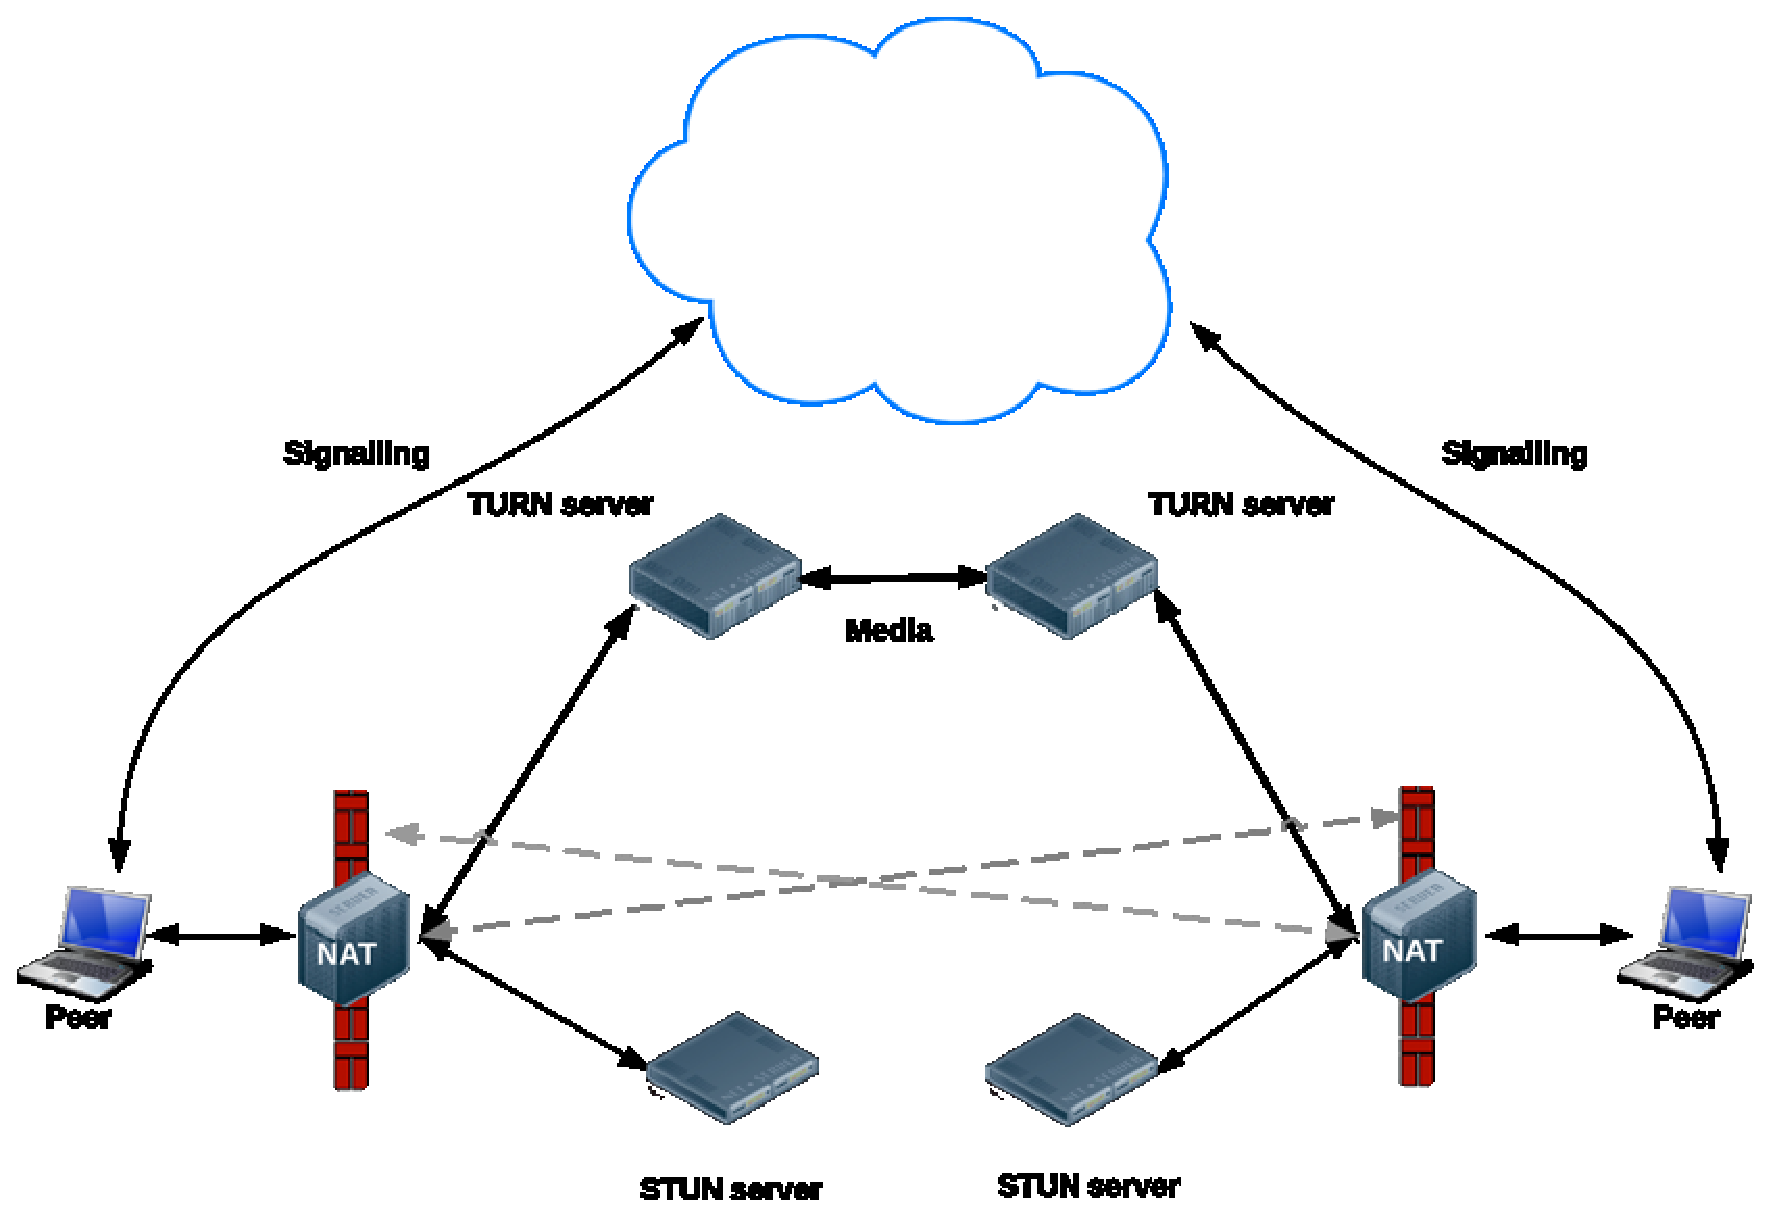
\includegraphics[width=0.8\columnwidth]{turn.eps}
	\caption{STUN, TURN et signalisation}
	\label{fig:turn}
\end{figure} 

La Figure \ref{fig:turn} représente le cas le plus complexe que l'on peut 
rencontrer pour établir une connexion WebRTC. Le plus simple des réseaux P2P 
peut être résumé comme deux machines connectées directement l'une à l'autre. 
Cette vision un peu utopique ne tient pas compte des routeurs qu'une connexion 
internet peut rencontrer. 
Chaque routeur peut posséder un \gls{NAT} afin de faire correspondre 
les adresse IP à d'autres adresse IP (dans le cas d'un intranet par exemple). 
Cela permet de faire communiquer des machines non uniques et non routables en 
faisant semblant d'utiliser des adresses externes, uniques et routables. 
Pour permettre à un client situé derrière un routeur \gls{NAT} de connaître son 
adresse IP publique et le type de serveur \gls{NAT}, l'utilisation d'un serveur 
\gls{STUN} est requise. 
L'utilisation d'une \gls{NAT} dynamique impose des restrictionq sur l'adresse de  
destination. Dans ce cas, le \gls{STUN} est inutile, on utilise un serveur 
\gls{TURN} qui est considéré comme une extension du \gls{STUN} et fait office de 
proxy. 
Une fois le client parvenu à récupérer une adresse IP, il peut participer à 
l'initialisation d'une connexion WebRTC (signalisation). L'utilisation de protocoles 
tels que \gls{ICE} avec son \gls{ICEF} permet de faciliter la mise en relation des 
clients derrière un \gls{NAT}. \gls{ICEF} choisi le chemin le plus cours entre les 
deux pairs et va utiliser le protocole adapté pour établir la connexion (\gls{STUN} 
d'abord puis en cas d'échec, \gls{TURN}).


%Du point de vue sécurité des communications, le standard requiert 
%obligatoirement le chiffrement pour tous les composants \gls{WebRTC}. 
%Cependant, les mécanismes de signalisation n'étant pas définis par le standard, 
%cela signifie que les développeurs sont assez libres d'utiliser les protocoles de 
%signalisation qu'ils souhaitent (SIP, \gls{WebSocket}, \gls{XHR}, une \gls{API} 
%externe\dots). Dans le cas où la connexion subit une attaque, la connexion peut 
%être stoppée, 
%redirigée ou enregistrée, altérée ou encore subir de l'injection de contenu. Pour 
%sécuriser la connexion l'utilisation de protocoles sécurisés comme HTTPS ou 
%\gls{WebSocket} (basé sur \gls{TLS}), assure qu'un message ne peut être 
%déchiffré.

\subsection{Quel protocole dans quel EVC3D ?}
%\improve{reformuler paragraphe}
Un des aspects prépondérant dans les \gls{EVC3D} concerne la communication et 
la transmission des données lors de la collaboration. Que ce soit dans dans un 
\gls{EV}, un jeu multijoueur ou un jeu sérieux (\textit{serious game}), les 
participants interagissent en temps-réel ou quasi-réel alors qu'ils sont situés à 
différents endroits géographiques. 
Le développement d'un \gls{EVC3D} nécessite donc des connaissances issues de 
plusieurs domaines comme la conception et l'implémentation de protocoles 
réseaux et de réseaux distribués.

Comme l'indique \cite{Roberto2014}, le protocole le plus souvent rencontré dans 
les \gls{EVC3D} est l'\gls{UDP}. 
Cette prépondérance s'explique d'après deux situations. Premièrement, dans des 
réseaux où l'accès est fiable car ces environnements n'ont 
pas (ou peu) de perte de paquet (ex : \gls{LAN}). Deuxièmement, dans un contexte 
d'application où la perte de paquet n'est pas critique (ex : jeu vidéo, diffusion en 
continu de son, vidéo, 3D\dots). 
\gls{UDP} peut également s'utiliser dans les tout type de réseaux -- \gls{LAN} ou 
\gls{WAN} (comme internet) --, car il est basé sur des datagrammes. Le fait qu'il 
n'effectue pas de vérification de délivrance lui donne un avantage quant 
à la taille des données envoyées dans les \glspl{EVC}. La responsabilité de 
vérifier quels sont les 
paquets qui n'ont pas été délivrés et leur ordre d'arrivée incombe à l'application.

\gls{TCP} est le protocole qui vient en seconde position. Les \gls{EVC3D} qui sont 
implémentés sur des réseaux haut-débit ne sont pas affectés par les étapes de 
vérifications que nécessitent une connexion \gls{TCP}. D'après \cite{Sung2006}, 
l'utilisation du protocole \gls{TCP} sur internet dans le cadre des \gls{EVC3D} n'est 
pas recommandée à cause de la taille de l'en-tête et du ACK qui réduisent le débit 
des paquets.
Dans ce contexte, le protocole \gls{UDP} obtient de meilleurs résultats dans le cas 
où le flux de données est local (\gls{LAN}). 
Les protocoles les plus adaptés pour communiquer dans un \gls{EVC3D} sont 
cependant \acrshort{SCTP} et \gls{RTP}/\gls{RTCP}. Ils combinent les 
fonctionnalités de 
\gls{TCP} et \gls{UDP} et sont optimisés pour les applications multimédia (flux et 
temps-réel). \gls{SCTP} offre la possibilité de choisir entre un système de 
livraison fiable (pour les paquets clés par exemple) ou non fiable (pour des mises 
à jour normales).

Depuis plusieurs décennies, les architectures \gls{P2P} sont utilisées dans les 
\gls{EVC}. Par exemple, l'assistance au rendu 3D par les pairs pour le rendu est une 
méthode qui permet aux pairs hébergés sur des appareils avec des capacités 
limitées (bande passante, processeur, processeur graphique) de demander une 
partie du contenu de l'environnement aux autres pairs.
Des systèmes récents comme celui de Martinez et al. \cite{Martinez2009} 
utilisent la 
localisation d'un utilisateur pour transmettre uniquement les mises à jours à son 
plus 
proche voisin. 
Ce système d'assistance par les pairs peut également être utilisé pour améliorer le 
rendu dans les environnements virtuels en ajustant la qualité du rendu en fonction 
du coût de calcul \cite{Zhu2011}.  
Koskela et al. \cite{Koskela2014} sont allés plus loin dans cette direction en 
proposant la méthode RADE (\textit{Ressource-Aware P2P-assisted 3D Delivery 
	Method}). RADE repose sur l'utilisation du \gls{P2P} pour alléger le chargement 
	et 
donc réduire le coût d'exploitation des fournisseurs de service. Les 
clients peuvent également être inclus en tant que fournisseurs de services dans 
cette architecture. 
Le système utilise un serveur qui connaît la localisation des ressources et 
effectue le \textit{load balancing} nécessaire pour distribuer les données en 
fonction des capacités des clients. L'impact énergétique d'un tel système a été 
évalué sur les mobiles ciblant trois optimisations possibles : la qualité visuelle, les 
performances et la consommation d'énergie. 

Les architectures hybrides, combinant client-serveur et \gls{P2P} sont également 
des solutions utilisées dans le cadre de l'apprentissage en ligne 
\cite{Ekadiyanto2012} et du BIM \cite{Chen2014} par exemple. 

En général, les systèmes \gls{P2P} semblent n'être supportés que dans les 
environnements virtuels 3D. Ce phénomène est probablement dû au lien étroit 
entre la séparation spatiale de l'utilisateur et le besoin de distribuer les données à 
tous les participants.
%
%
%	\subsection{Introduction}
%	\subsection{Les approches centralisées}
%	\subsection{Les approches décentralisées}
%	\subsection{Conclusion}

%\section{Systèmes d'édition collaborative}
%	\subsection{Le modèle de cohérence CCI}
%	\subsection{Les approches pour les données 3D}
%	\subsection{Conclusion}

\section{Les systèmes distribués orientés événements pour la collaboration}

	\subsection{Introduction}
% old evenements et collaboration
La plupart des systèmes basés événements sont très populaires lorsqu'il s'agit de 
collaboration\cite{Helmer2011}. Les événements peuvent être utilisé dans 
\gls{CSCW}
On retrouve par exemple la spécification 
d'événements composites 
pour le support de la collaboration dans la conception logicielle \cite{Yuan2002} 
ou encore la définition de patrons de conception dédiés à la collaboration dans les 
architectures basées événement \cite{Verginadis2009}. Dans ce dernier domaine 
Papageorgiou et al. \cite{Papageorgiou2011} proposent un assistant à la 
création de ces patrons dédiés à la collaboration. Ils s'appuient sur un système de 
recommandation basé sur le contexte qui utilise une représentation sémantique 
(\gls{OWL}).

CoDesign est un exemple de \gls{framework} permettant de faire de la 
conception logicielle de manière collaborative \cite{Bang2010}. L'utilisation d'une 
architecture basée événement permet à l'application d'être très extensible car très 
peu couplée. Chaque instance CoDesign intègre un intergiciel appelé CoWare en 
charge de la synchronisation de contenus édités de manière concurrente sur les 
différentes instances CoDesign, ainsi qu'un module chargé de notifier les 
architectes de situations de modélisation conflictuelles. 


Eventuate est une plateforme qui se base sur un modèle de programmation 
événementielle ayant pour but de résoudre les problèmes liés à la gestion de 
données distribuées inhérents aux architectures microservices en utilisant \gls{ES} et
\gls{CQRS}. Une de leurs applications exemple est un tableau Kanban collaboratif 
temps-réel construit sur leur 
plateforme\footnote{https://github.com/eventuate-examples/es-kanban-board}. 
%	\subsection{Les événements comme base du comportement réactif}
	\subsection{Systèmes Publish-Subscribe}

Le système \glsreset{PubSub}\gls{PubSub} est un mécanisme basé sur le 
paradigme des 
messages qui est beaucoup utilisé en Event Processing. 
Les \textit{publishers} (ceux qui émettent des messages) et les \textit{subscribers} 
(ceux qui souscrivent) sont couplés de manière lâche. 
Autrement dit, le \textit{publisher} n'est pas forcément au courant de l'existence de 
ses \textit{subscribers} et n'a donc pas de contrainte forte le liant à ces derniers. 
De son côté, le \textit{subscriber} est souvent indifférent au \textit{publisher} qui lui 
fournit les événements qui l'intéressent. La Figure \ref{fig:pubsub} représente le 
modèle \gls{PubSub}.
Le service de notification d'événement est utilisé comme passe-plat d'événements 
entre le publisher et les subscribers. Son rôle est de gérer les abonnements 
(souscription / désinscription) et de notifier les \textit{subscribers} concernés par la 
publication d'un événement par un \textit{publisher}.
%TODO expliquer la figure 

\begin{figure}[ht!]
	\centering
	\inputTikZ{1}{eps/tikz/pubsub}
	\caption{Architecture Publish-Subscribe}
	\label{fig:pubsub}
\end{figure}


Les modèles utilisant le paradigme \gls{PubSub} supportent naturellement une 
communication \textit{many-to-many} 
entre les publieurs (\textit{publishers}) et les souscripteurs (\textit{subscribers}).  De cette manière, le meilleur passage à l'échelle d'une application est facilité grâce à une topologie du réseau plus flexible. 


Pour répondre à des besoins de mise à l'échelle, d'interopérabilité, de fiabilité, 
d'expressivité et d'utilisabilité, il s'appuie sur un modèle \gls{PubSub} basé types 
et attributs. 
En spécifiant d'abord le type et ensuite en filtrant sur les attributs des 
événements, ce modèle rend le routage des données intuitif pour le 
développement d'applications distribuées à grande échelle comme le commerce en 
ligne (\textit{e-commerce}). 
Scribe \cite{Castro2002} et Hermes \cite{Pietzuch2002} sont des exemples de 
systèmes \gls{PubSub} basés sur les \glspl{DHT}. 
Le premier se concentre sur la catégorie du sujet (topic-based) tandis que le second 
supporte à la fois la communication orientée sujet et la communication orientée contenu (content-based) en utilisant un 
filtrage par agrégat. Les deux utilisent un n\oe ud \textit{rendezvous} pour chaque 
sujet ou type d'événement dans la couche réseau et construisent et maintiennent la 
distribution à partir de ce n\oe ud \textit{rendezvous}. TERA \cite{Baldoni2007} 
propose une dissémination sur deux couches orientée sujet. Le but est d'effectuer 
une distribution uniforme en fonction des intérêts des n\oe uds. La dissémination 
se déroule en deux phases. Pendant la première phase, un algorithme de marche aléatoire (succession de pas aléatoires dans le graphe)
est utilisé sur la couche basse qui connecte les n\oe uds dans le but de localiser 
le n\oe ud qui a souscrit au sujet. La seconde phase commence lorsqu'un 
\textit{subscriber} est trouvé pour le connecter au \textit{cluster} correspondant au 
sujet sur la couche haute. C'est là que l'événement est disséminé.

En juin 2017, Leonardo Quernozy présente une rétrospective des systèmes 
\gls{PubSub} en \gls{P2P} massifs lors de la conférence DEBS'2017 à 
Barcelone. 
Les premières traces d'une telle architecture remontent à 1987 avec 
la publication de Birman et Joseph \cite{Birman1987} lorsqu'ils évoquent \og 
the ''News'' service in the ISIS system\fg{}:

\blockcquote{Birman1987}{
	\og\textit{ This service allows processes to enroll in a 
		system-wide news facility. Each subscriber receives a
		copy of any messages having a "subject" for which it 
		has enrolled in the order they were posted. Although 
		modeled after net-news, the news service is an active 
		entity that informs processes immediately on learning 
		of an event about which they have expressed interest.}\fg{}
}

Après cette publication, les premiers systèmes \gls{PubSub} commencent à 
se développer. Le concept de routeur d'information est introduit par Oki et al. 
\cite{Oki1993} : un seul bus d'information pour tous les services, objets, données
\ldots Les protocoles de communication ont une sémantique minimale, 
les objets (instances de classe) sont auto-descriptifs - i.e. ils sont 
capables d'introspection (service, opérations, attributs) pour adapter leur 
comportement au changement, les types peuvent être définis dynamiquement et 
la communication est anonyme. 
Puis des solutions plus avancées sont apparues avec le projet 
GRYPHON d'IBM \cite{Banavar1999}, SIENA \cite{Carzaniga2000}, REBECA 
\cite{Parzyjegla2010} et également REDS, JEDI, PADRES présentés plus en 
détails dans \cite{Tarkoma2012}.
Ces différentes solutions ont été conçues comme des systèmes de gestion avec 
des gestionnaires d'événements dédiées. Le passage à l'échelle est 
principalement effectué par un routage efficace des événements (comme le 
filtrage d'événements). Seuls quelques travaux ont utilisé le concept de 
\textit{clustering} par intérêt comme moyen afin de réduire le nombre de 
notifications d'événement et éviter la surcharge. 
A partir des années 2000, les 
systèmes \gls{P2P} ont commencé à émerger avec 
l'apparition de Gnutella et consorts, les \glspl{DHT} (Chord, Pastry, Kademlia) et  
Réseaux non-structurés (Cyclon, Scamp, ADH). Ces systèmes ont pour 
objectif de gérer des réseaux massifs, dynamiques (\textit{churn}), résistants 
aux 
erreurs, et offrants des primitives de communications basiques.
Les réseaux \gls{P2P} promettent alors des propriétés intéressantes pour les 
infrastructures logicielles comme les systèmes \gls{PubSub} concernant le passage à 
l'échelle. Cependant, les systèmes \gls{PubSub} d'alors reposent sur une connaissance 
totale du réseau pour être efficaces, du fait de leur taille limitée. La connaissance 
globale de l'information ne peut être collectée dans un système à grande échelle, 
c'est pourquoi la décentralisation de l'information est nécessaire. La connaissance 
peut vite devenir viciée dans un système dynamique décentralisé, ce qui implique 
de trouver une méthode efficace pour gérer la dynamicité.

Les systèmes \gls{PubSub} ont donc l'avantage de proposer une \gls{EDA} dont le 
fonctionnement s'adapte à plusieurs types de communication, que ce soit client 
serveur, P2P. Cette flexibilité a l'avantage de proposer un système à couplage 
lâche qu'il reste cependant difficile d'observer à grande échelle.

\subsubsection{Outils de surveillance, contrôle de performances et validation ergonomique}
Dans un système distribué comme \gls{PubSub}, les outils de comparaison 
sont souvent très hétérogènes et ne permettent pas forcément d'évaluer sur une 
même base la montée en charge. 
Carzaniga and Wolf \cite{Carzaniga2002} proposent quelques 
lignes directrices pour concevoir une suite de \textit{benchmark} dans un système 
\gls{PubSub}, sans fournir de résultat spécifique, dont le but est double : la 
validation de l'interface et l'évaluation de la performance. 
La pertinence de l'interface a été définie par une série de questions/réponses 
posée au développeur. Elle adresse plusieurs aspects liés à l'\gls{IU} : 
\begin{itemize}
	\item le modèle de publication (structure, domaines de valeur, taille des objets);
	\item le modèle de souscription (portée de l'évaluation d'une publication reçue, 
	type de langage, expressivité du langage pour la sélection);
	\item les méthodes d'accès à l'interface (accès local, mémoire partagée) ; 
	\item la portabilité du système (support multi-plateforme) ;
	\item le type de service (fiabilité) et les fonctionnalités auxiliaires. 
\end{itemize}

Pour évaluer la charge de travail d'un système distribué basé événements, 
Kounev et al. \cite{Kounev2008} ont utilisé des techniques d'analyse 
opérationnelle pour caractériser le trafic du système et dériver une approximation 
de la moyenne des délais de livraison d'événements. 

%TODO precisier quelles recherches
Beaucoup de recherches ont été menées dans le but d'améliorer les performance 
des systèmes collaboratifs utilisant une architecture distribuée. Bien que ces 
approches permettent de passer à l'échelle de grandes quantités de données, cela 
requiert de lourds investissement pour installer et maintenir plusieurs serveurs 
dédiés. Une alternative à bas coût est d'utiliser les différents clients à disposition 
(qui sont en relation par le biais de la collaboration) pour avoir un traitement réparti 
des données sur la foule (\textit{crowd computing})\cite{Li2015}. De ce fait, le 
contenu 3D est distribué par les pairs et non plus par le serveur. En combinant les 
ressources réseau du serveur et de plusieurs clients, on peut réaliser une 
distribution des données (événements) en améliorant les performances du 
système pendant les sessions de travail collaboratif. 




\subsection{Domain Driven Design}
%\subsection{Domain Driven Design : lier le fonctionnel et le code}
	
	\glsreset{DDD}\gls{DDD} ou Conception Pilotée par le Domaine est une 
	approche de 
	développement logicielle qui a pour objectif de définir une vision et un 
	langage partagé (\textit{ubiquitous language}) pour les personnes 
	impliquées dans la construction d'une application \cite{Evans2003}.
	Avec le \gls{DDD}, un projet est vu a travers le prisme du domaine d'application qui le concerne (métier) et la logique du domaine en basant des conceptions complexes sur un modèle du domaine. Cela s'inscrit dans l'objectif d'initier une collaboration créative entre les experts techniques et les experts du domaine pour produire un modèle conceptuel -- qui relève de problèmes spécifiques au domaine -- raffiné itérativement.
	Les différents concepts du \gls{DDD} sont listés en suivant :
	\begin{description}
		\item[Le contexte] est le cadre dans lequel un mot apparaît qui détermine sa 
		signification ;
		\item[Le domaine] est une ontologie, une influence, ou une activité. 
		L'étendue du sujet auquel l'utilisateur applique un programme est le domaine 
		du logiciel ;
		\item[Le modèle] est un système d'abstractions qui décrit les aspects 
		sélectionnés du domaine et qui sont utilisés pour résoudre les problèmes liés 
		à ce domaine ;
		\item[Le langage partagé] est un langage structuré autour du modèle du 
		domaine utilisé par tous les membres de l'équipe pour faire référence aux 
		activités de l'équipe permettant d'éviter la redondance et les ambigüités dans
		un contexte donné.
	\end{description}

\begin{figure}
	\noindent
	\centering
	\includegraphics[width=0.9\columnwidth]{ddd.eps}
	\caption[Illustration du patron \gls{DDD} et de ses artefacts]{Illustration du 
	patron \gls{DDD} et de ses artefacts (issue de 
	\cite{Avram2006} sous licence Creative Commons)}
\label{fig:ddd}
\end{figure}

Le \gls{DDD} permet de connecter le modèle et son implémentation en offrant 
plusieurs avantages. La plasticité du système est mise en avant par l'expression 
de règles et de comportements qui facilitent les changements fréquents.
L'accent mis sur l'identification des interactions dans le système encourage la 
mise en \oe{}uvre d'une interface orientée tâches (\textit{task-based UI}).
La testabilité fonctionnelle est intégrée via les règles métier explicitées 
et concentrées dans une couche spécifique de l'application. Cela les rend 
plus facilement identifiables et testables automatiquement.
La robustesse est améliorée face aux changements dans le système d'information.

En \gls{DDD}, il existe des artéfacts qui permettent d'exprimer, créer et stocker un 
modèle lié à un domaine (voir Figure \ref{fig:ddd}). Parmi les principaux se trouvent 
:
\begin{itemize}
	\item L'\textbf{entité} (\textit{entity}) : un objet qui n'est pas défini par ses 
	attributs 
	mais plutôt par une continuité et son identité. 
	Par exemple, chaque scène possède des maillages qui utilisent des 
	géométries.Si l'on 
	considère un maillage comme unique dans chacune des scènes alors chaque 
	maillage est une entité. Si on considère que ce sont les mêmes maillages qui 
	sont réutilisés alors un maillage est considéré comme un objet-valeur.
	
	\item L'\textbf{objet-valeur} (\textit{value object}) : un objet qui contient des 
	attributs 
	mais n'a pas d'identité conceptuelle. Il doit être traité comme un objet
	immuable. Par rapport à l'exemple précédent, on peut considérer que si les 
	géométries sont réutilisées d'une scène à l'autre, ce sont des objets-valeurs qui 
	ne seront jamais modifiés car les utilisateurs ne sont intéressés que par les 
	informations qu'elles portent.
	
	\item L'\textbf{agrégat} (\textit{aggregate}) : une collection d'objets qui sont 
	liés 
	ensemble par une entité commune (\textit{root entity}), connue sous le nom 
	d'agrégat souche (\textit{aggregate root}). Ce dernier garantit la cohérence des 
	modifications faites au sein de l'agrégat en interdisant aux objets externes de 
	faire référence à ses membres. Par exemple, dans une modélisation 3D 
	collaborative un utilisateur ne peut pas modifier le nom d'un autre utilisateur. Un 
	maillage n'a également pas d'intéret à connaître les informations des 
	utilisateurs, c'est la scène qui gère l'interface entre les maillages et les 
	utilisateurs.
	\item L'\textbf{événement du domaine} (\textit{domain event}) : un 
	événement auquel 
	l'expert du domaine s'intéresse. Il est définit par un objet du domaine.
	\item Le \textbf{dépôt} (\textit{repository}) : les méthodes pour récupérer les 
	objets du domaine doivent être déléguées à un \textbf{dépôt} spécialisé afin de 
	faciliter les implantations 
	alternatives de stockage.
\end{itemize}



Les notions plus détaillées qui se rapportent au \gls{DDD} sont présentées dans 
\cite{Evans2003} et \cite{Vernon2013}\footnote{Les différents ouvrages publiés par 
Vernon s'attachent également à montrer la nécessité pour les différentes 
branches de l'informatique à proposer des 
systèmes d'information plus robustes et flexibles face aux nouvelles demandes.}.\info{source: 
	http://blog.octo.com/domain-driven-design-des-armes-pour-affronter-la-complexite/}

Le \gls{DDD} a également l'avantage de fonctionner en harmonie avec les 
principes de l'\gls{ES}. L'approche logicielle \gls{DDD} étant conçue pour refléter 
les événements se déroulant dans la réalité métier qui ne sont pas 
interchangeables -- la plupart du temps. L'utilisation d'architectures 
basées événements est naturelle dans ce genre d'environnement. 

Les disciplines liées à la 3D dans un contexte industriel ont besoin de pouvoir 
communiquer sur un langage partagé pour permettre à chacun des 
intervenants de s'exprimer dans la création du produit. Par exemple, la \gls{CAO} 
est très utile dans un contexte d'ingénierie grâce à l'utilisation de quatre propriétés 
fondamentales telles que l'historique, les fonctionnalités, la paramétrisation et le 
haut niveau de contrainte.



\subsection{Command Query Responsability Segregation}
%	\subsection{Command Query Responsability Segregation : garantir de 
%	l'intégrité 
%	des données }
\label{sec:CQRS}
Une solution architecturale courante en \gls{DDD} contient quatre 
couches : l'interface utilisateur (présentation), la couche application (coordination 
de l'activité de l'application), la couche domaine (c\oe ur du logiciel métier), la 
couche infrastructure (interface entre les couches, persistance des objets 
métier\dots). La Figure \ref{fig:dddcqrs} montre que ces quatre couches s'accordent
bien avec l'architecture \gls{CQRS} qui sépare le flux d'écriture et de lecture dans 
le logiciel.

Introduit par Greg Young en 2009 \cite{Young2009}, \gls{CQRS} est un patron de 
conception qui repose sur le principe de séparation des composants de traitement 
métier de l'information (écriture) et de la restitution de l'information (lecture). Le 
cadre offert par ce principe permet de lever certaines contraintes d'architecture 
comme le passage à l'échelle en faisant apparaître de nouvelles forces : la gestion 
de la concurrence dans la collaboration sur des règles métier propre à la 
modélisation 3D dans des cadres d'application spécifiques. En effet, selon le type 
d'application, un ensemble de règles régit les droits concernant les types de 
modifications acceptables et qui est autorisé à le faire.

\begin{figure}[ht]
	\noindent
	\centering
	\inputTikZ{1}{eps/tikz/ddd/dddcqrs}
	\caption{Architecture en 4 couches du DDD (gauche) en miroir avec 
		l'architecture CQRS 
		(droite)}
	\label{fig:dddcqrs}
\end{figure}


Le caractère vicié (\textit{staleness}) d'une donnée dans un environnement 
collaboratif est récurrent. Une fois que la donnée a été montrée à un utilisateur, la 
même donnée peut être changée par un autre utilisateur, elle est altérée. 
\gls{CQRS} pallie cela en répondant aux besoins suivants :
\begin{itemize}
	\item \textbf{En traitement / écriture} : besoins transactionnels, garantie de cohérence 
	des données, de normalisation ;
	\item \textbf{En consultation / lecture}: dénormalisation, passage à l'échelle.
\end{itemize}

La plupart des architectures en couches ne font pas explicitement référence à ces 
problèmes. Le fait de tout sauvegarder dans une base de données centralisée peut 
être une étape dans la gestion de la collaboration, mais l'altération des données est 
souvent exacerbée par l'utilisation de caches comme accélérateur de performance.
L'immuabilité en \gls{CQRS} est un concept clé qui prévient la  
modification de l'état interne d'une commande ou d'un événement. Les 
commandes sont immuables car leur usage nécessite un envoi direct au domaine 
pour être traitées. Quant aux événements, ils sont immuables car ils représentent 
ce qui s'est produit dans le passé (qu'on ne peut donc pas changer). 

\subsection{Event Sourcing}
%\subsection{Event Sourcing : certifier la fiabilité et traçabilité des données}
\label{sec:es}

Le Reactive Manifesto, apparu en 2014, est un document qui résume les 
propriétés clés liées aux systèmes distribués et encourage notamment le 
développement de systèmes \og plus flexibles, à couplage faible et 
extensibles\fg{}\cite{Boner2014} comme le \gls{CQRS} et l'\gls{ES}.

L'\glsreset{ES}\gls{ES} est une approche complémentaire au \gls{CQRS} pour 
gérer la 
concurrence des données et capturer l'intention de l'utilisateur. Ce patron de 
conception stocke les événements en mode ajout seulement 
(\textit{append-only}) pour sauvegarder le résultat des commandes sur le 
domaine. Cela permet de conserver tous les changements qui ont mené à un 
état plutôt qu'uniquement l'état. Ce paradigme permet de recréer n'importe quel 
état d'un agrégat à partir de la liste d'événements qu'on lui a appliqué. Cette 
liste représente une base la vérité du système\jp{pas clair}. 
\improve{improve}\gls{ES} permet de simplifier les tâches complexes dans des 
domaines complexes comme la 3D en ne requérant pas la synchronisation de 
modèle de données et du métier. 

L'\gls{ES} est souvent présent dans des architecture asynchrones qui ont 
l'avantage de pouvoir utiliser des queues de message, plusieurs bases de 
données, et où la partie lecture est éventuellement consistante.
La plupart de la littérature concernant ce patron se trouve en ligne, dans des 
billets de blog, des présentations ou de la documentation logicielle. La 
littérature académique est relativement réduite et se rapporte principalement
à l'étude de l'évolution de graphes dans le temps \cite{Erb2015,Erb2017}. Cette section fournit un aperçu des différentes 
définitions données de l'\gls{ES} et du vocabulaire lié à ce patron de conception.

Martin Fowler a été le premier à utiliser le terme 
d'\acrlong{ES} en 2005. Il définit l'\gls{ES} comme \og une série de 
changements 
de l'état d'une application\fg{}. Il voit les événements 
comme immuables et le journal d'événement (\textit{event log}) comme un 
stockage linéaire (\textit{append only store}) des événements (Figure 
\ref{fig:es-event}). 
Les événements ne sont jamais supprimés, le seul moyen de l'''annuler'' consiste à 
effectuer générer un événement rétroactif. 
Une fois qu'un événement rétroactif est ajouté, l'événement rétroactif agit à 
l'inverse de l'événement précédent pour compenser ses effets (Figure 
\ref{fig:es-transaction-delete}). 
Dans ce billet, Fowler n'établit pas clairement la distinction entre les 
événements 
et les commandes qui déclenchent ces événements. Ce problème est 
considéré dans plusieurs travaux fondamentaux \cite{Prakash1994,Sun2002,Weiss2009a,Weiss2010}, et approfondi par une revue de Chen et al. \cite{Cheng2013}.

Greg Young, important contributeur au domaine de l'\gls{ES} (et \gls{CQRS}), décrit l'\gls{ES} comme \og le stockage de l'état courant sous la forme 
d'une série d'événements et la reconstruction de l'état du système en rejouant 
cette série d'événements\fg{}. D'après lui, le journal d'événements a également 
un comportement linéaire : les événements qui sont déjà arrivés ne peuvent 
être défaits. Ce que Fowler appelle événements rétroactifs, Young le décrit 
comme des actions inverses.

\textbf{Udi Dahan} Udi Dahan est également un auteur de billets de blog 
prolifique sur les systèmes \gls{ES}. Dans sa définition de l'\gls{ES}, Dahan 
insiste sur le fait que \og l'état du modèle du domain est persisté comme un 
\textit{flux} d'événements plutôt qu'un simple instantané\fg{}.


%
	\begin{figure}[!h]
		
		\centering
		\noindent
		\subfloat[Nouvel événement en \gls{ES}]{
			\inputTikZ{1}{eps/tikz/eventsourcing/es.tex}
			\label{fig:es-event}
		}
	
	\subfloat[Transaction avec compensation en \gls{ES}]{
		\inputTikZ{1}{eps/tikz/eventsourcing/escompensation.tex}
		\label{fig:es-transaction-delete}
	}
		\caption{Transaction en \gls{ES}}
		\label{fig:es-transaction}
	\end{figure}

	
	\begin{figure}[t]
		\centering
		
		\subfloat[Sans la notion de Snapshot]{
			\includegraphics[width=0.4\textwidth]{without-snapshot.eps}
			\label{fig:es-without-snapshot}
		}
		\subfloat[Avec la notion de Snapshot]{
			\includegraphics[width=0.4\textwidth]{snapshot.eps}
			\label{fig:es-snapshot}
		}
		\caption{Snapshot en \gls{ES}}
	\end{figure}

Les avantages et les inconvénients de l'approche \gls{ES} dépendent du
cadre dans lequel elle est utilisée. En reprenant ceux cités par Klamer 
\cite{Klamer2013a}, ils peuvent être envisagés sous l'angle de la modélisation 3D 
collaborative.

\subsubsection{Avantages}
L'\gls{ES} peut apporter beaucoup d'avantages à une application, notamment 
lorsque les besoins en traçabilité de l'information sont importants comme dans 
la modélisation collaborative de données 3D.
L'historique du système est accessible tout au long de la vie de l'application, ce 
qui implique qu'il est non seulement possible d'accéder à l'état courant du 
système, mais également à toutes les actions ayant mené jusqu'à cet état. C'est 
un avantage certain pour les système critiques, les applications d'Informatique 
Décisionnelle ou les applications collaboratives. La pratique la plus 
courante est de proposer un système principal et d'ajouter une multitude de 
sous-systèmes qui enregistrent les différentes métriques (analyse d'un ou 
plusieurs axes, \textit{reporting} sur une propriété) du système principal. Avec 
l'\gls{ES}, il est toujours possible de regarder \og dans le passé\fg{} et de 
récupérer les données à partir de ce moment. Par comparaison, les avantages de 
l'\gls{ES} sur l'Active Record sont:
\begin{itemize}
	\item un journal complet de tous les changements d'état,
	\item une traçabilité et un débogage efficace,
	\item de très bonnes performances,
	\item pas de mapping objet-relationnel (ORM)\info{citer fowler's book}.
\end{itemize}

	
\paragraph{Exemple} 
Une revue de projet d'une scène est effectuée dans le cadre d'une application 
collaborative de modélisation 3D en ligne. Le chef de projet remarque qu'un 
objet a subi énormément de modifications par rapport aux autres. Il examine en 
particulier cet objet pour en connaître les causes. Voici deux exemples 
d'observations possibles : 1/ les spécifications ne sont pas assez claires 2/ 
deux collaborateurs sont opposés sur la façon de modifier l'objet. L'origine de 
ces changements identifiée, le chef de projet pourra alors intervenir et clarifier 
le sujet. \improve{style exemple}

\paragraph{Résolution} Avec un système classique, la fonctionnalité doit être 
créée pour enregistrer ce traitement, puis être testée et implémentée (dans cet 
exemple, il en faudrait deux). Ensuite seulement, un rapport pourra être délivré. 
Dans un environnement utilisant l'\gls{ES}, tous les événements existent déjà 
donc les données sont déjà disponibles et ont seulement à être analysées 
(dans notre exemple, les informations sont inhérentes aux événements). De plus, 
les événements étant stockés depuis le début de la vie -- mise en route -- de l'application , beaucoup plus de données peuvent être analysées. Par 
exemple : demander toutes les modifications d'un objet depuis la dernière 
connexion d'un utilisateur pour lui communiquer visuellement les différences par 
rapport à sa dernière visite.



\subsubsection{Inconvénients}
En revanche, les performances de l'application peuvent être affectées par 
l'utilisation de 
l'\gls{ES}. En effet, pour récupérer l'état courant à partir de l'Event Store, il est 
nécessaire de le calculer à partir des événements reçus.
A chaque événement créé (et stocké), ce processus sera alourdi car ils ne 
peuvent être supprimés. Plus la pile d'événements est longue, plus cela prend 
du temps (linéaire), considérant que les commandes ont parfois besoin de connaître une
partie de l'état courant issu de ces événements pour être déclenchées.
 
Un \gls{snapshot} est une capture de l'état de l'agrégat à un 
moment qui correspond à l'empilement d'événements ayant mené à cet état. En 
créant un \gls{snapshot}, on évite de reconstruire un état à partir du début de la 
vie de l'agrégat (Figure \ref{fig:es-without-snapshot}) ; on empile les nouveaux 
événements à partir de ce snapshot (Figure \ref{fig:es-snapshot}). 
L'utilisation du \gls{snapshot} est intéressante à partir du moment où la pile 
d'événements devient plus lourde que le \gls{snapshot} lui-même. Il est donc 
important de bien déterminer la périodicité du déclenchement du \gls{snapshot} 
(temporelle ou selon le nombre d'événements).
 \info{rehydratation d'un agrégat diff avec projection -> eventually consistence (proj 
 = EC /rehy -> 
	valides}\unsure{Dans tous les autres cas l'utilisation de \textit{snapshots} 
	permet de contrer proprement ce problème en offrant une forme dénormalisée 
	de la donnée. }

Le parcours des événements se fait classiquement du premier au dernier 
(\textit{bottom-up}). Si on utilise les \gls{snapshot}, on peut se permettre de les 
parcourir dans l'autre sens (\textit{top-bottom}) jusqu'à trouver un \gls{snapshot} 
puis appliquer tous les événements qui sont arrivés entre ce \gls{snapshot} et 
l'état courant. Pour accéder à des données historiques 
plus anciennes que le dernier \gls{snapshot}, le second parcours fonctionne 
aussi. Cependant, il doit être évitée pour ne pas créer de dépendance entre 
les \gls{snapshot}. Sans les snapshots le modèle peut encore varier 
<<~librement~>> tant que l'on sait comment lui appliquer un événement passé. 
Le fait de travailler avec des \gls{snapshot} crée une dépendance des 
snapshots qui doivent intégrer les modifications du domaine. Une solution est 
de recalculer les snapshots quand le domaine est modifié mais cela reste 
coûteux (et à éviter).\info{versionning event -> retro compatibilité}

\paragraph{Event Sourcing versus Command Sourcing}
Les patrons de conception \gls{CS} et \gls{ES} sont strictement déterministes pour 
avoir une exactitude rigoureuse de ce qui se passe dans le système.

Un événement représente quelque chose qui est arrivé dans le domaine. Un 
événement appliqué sur un état, donne un nouvel état. 
La condition pour appliquer un pur déterminisme en \gls{ES} est la fonction 
suivante : \texttt{État~$\rightarrow$~événement~$\rightarrow$~État}. 
Cette fonction met en correspondance les (mêmes) entrées avec les (mêmes) 
sorties ; ce qui permet de se reposer dessus pour reconstituer un état à 
n'important quel moment dans le temps. 
Le déterminisme est appliqué en assurant à l'événement tous les 
informations lui permettant de faire la transition (i.e. sans effet de bord). 
L'événement est alors considéré comme une encapsulation de toutes les 
informations pertinentes concernant la transition du système d'un état à l'autre.

Une commande va être déclenchée par l'utilisateur qui veut modifier le domaine. 
Une commande appliquée sur un état va produire un ou plusieurs événements (qui 
ne sont pas forcément appliqués à l'état courant de l'application par la suite): 
\texttt{État~$\rightarrow$~Commande~$\rightarrow$~Liste d'événements}.

La différence principale entre un événement et une commande réside donc dans 
l'\textbf{intention}. D'un point de vue fonctionnel, le \gls{CS} est un patron de 
conception lié à une décision qui produit plusieurs événements, tandis que 
l'\gls{ES} se contente d'appliquer un changement à l'état courant. De plus, en 
\gls{ES}, l'événement stocké a été produit par l'agrégat. 
La différenciation majeure des deux patrons de conception s'accentue lors de 
l'interaction avec des systèmes externes. L'aspect fonctionnel de l'application de 
changement d'état de l'\gls{ES} a l'avantage de permettre de reconstruire l'état sans 
effet de bord car elle ne travaille que sur l'état interne de l'application. 

Historiquement, l'\gls{ES} de Fowler dans ses premières versions ressemblait plus 
à du \gls{CS}. L'évolution de l'\gls{ES} a conduit à revoir ce patron théoriquement 
sous une forme fonctionnelle pure, avec l'apparition, par exemple, de bases de données fonctionnelles comme EventStore ou de langages de programmation plus adaptés comme F\#. Les deux 
patrons peuvent cohabiter si le \gls{CS} a un cadre d'action bien délimité 
et que les composants de l'architecture ont un couplage lâche afin que seuls les 
événements produits par les agrégats ne modifient l'état interne de l'application. 

\section{Conclusion}

La manipulation et la visualisation d'objets 3D sur le web est une problématique 
qui peut se découper en différentes parties.
La première concerne la modélisation collaborative 3D sur le web. Les plateformes 
existantes essayent de répondre à plusieurs challenge : conserver la cohérence 
de l'environnement, proposer des solutions performantes et économiques (bande 
passante, énergie, graphique, stockage)  pour s'adapter aux évolutions du web.
L'un des aspects fondamentaux du web est l'accessibilité. Cela passe par la 
standardisation des technologies web par le \gls{W3C}.  L'émergence des 
standards comme WebGL (affichage 3D) et WebRTC (connexion P2P entre 
navigateurs) a fait apparaître de nouvelles possibilités concernant la visualisation 
et le partage de données 3D. 


La seconde partie concerne la communication en temps réel au sein d'une 
application collaborative. Il existe plusieurs critères pour choisir le protocole de 
transport adapté à un \gls{EVC3D} : la fiabilité, l'ordonnancement et le risque 
d'erreur. 
Jusque là souvent cantonnés aux traditionnelles 
applications client-serveur sur web, les \glspl{EVC} se montrent malgré tout 
intéressés par les architectures de communications P2P (éventuellement 
combinées à une architecture client-serveur). Dans ce cadre, les \gls{EVC3D} 
particulièrement lors d'édition collaborative de scènes 3D, le choix d'une 
architecture \gls{P2P} combiné à la haute fréquence des mises à jour, suggère le 
choix d'un mode non fiable, non ordonné et sans erreur. C'est l'application qui gère 
les 
paquets manquants et leur ré-ordonnancement pour favoriser la rapidité 
de la livraison.

La troisième partie s'intéresse aux propriétés des architectures orientées 
événements ou \gls{EDA}. Le couplage lâche est une propriété 
qui s'accorde bien avec les systèmes distribués \gls{P2P} ou hybrides. Les 
\glspl{EDA} ont l'avantage de proposer une intégration de la partie métier 
transparente. Dans les différents systèmes de modélisation 3D pour la 
visualisation ou la manipulation d'objets 3D collaboratifs sur le web, 
cet aspect est souvent mis de côté. Or dans le cadre de 
la \gls{CAO}, du \gls{BIM} ou d'application au cadre industriel, ces points sont 
prépondérants.
Différentes approches parmi les architectures orientée événements dans un 
système collaboratif permettent d'intégrer les règles liées au métier dans une 
application de modélisation collaborative. Dans un 
premier temps, l'architecture \gls{PubSub} propose un système de notifications 
pour les différents 
n\oe uds d'un réseau de manière lâche. De cette manière, la communication est 
homogénéisée et repose uniquement sur des notifications d'événement pour les 
entrées et sorties des clients. Le mécanisme d'abonnement autorise une 
grande variété de stratégies quant au routage des messages.
Dans un second temps, différents patrons de conceptions sont présentés. Le 
\gls{DDD} est plutôt considéré comme un patron de conception stratégique. Ses 
principes permettent de donner au logiciel une vision orientée métier. 
A partir de ces orientations, \gls{CQRS} vient proposer une discrimination entre la 
partie écriture (commande) et lecture (requête) dans l'application. Le passage à 
l'échelle côté lecture est favorisé grâce à la création de projections des données. Elles facilitent la restitution des données sans risques d'effets de bord. 
Le côté écriture permet de valider le contenu entrant selon les règles métiers du domaine. L'\gls{ES} est le patron qui introduit la notion d'événement (\og 
ce qui s'est passé\fg{}). L'état de l'application se reconstruit à 
partir de ces événements issus de l'expertise métier -- déduite grâce au \gls{DDD}. 
Les événements générés par \gls{CQRS} sont stockés dans le journal des 
événements qui les partage aux autres collaborateurs, ce qui peut 
provoquer des conflits qu'il faut pouvoir détecter pour éviter les incohérences dans 
l'\gls{EVC}. 
%\todo{parler de la concurrence} 

